%! TEX root = ../main.tex
\chapter{An Interesting Chapter}\label{chap:intro}

  \lipsum{}

  \section{Demponstration}

    \subsection{Citing something}

      Citing something~\cite{darwin1909origin}.

    \subsection{Figures}

      See \Cref{fig:cat-and-dog}. Specifically, note the cat in \cref{fig:cat} and the dog in \cref{fig:dog}.

      \begin{figure}
        \centering
        \begin{subfigure}[b]{4cm}
          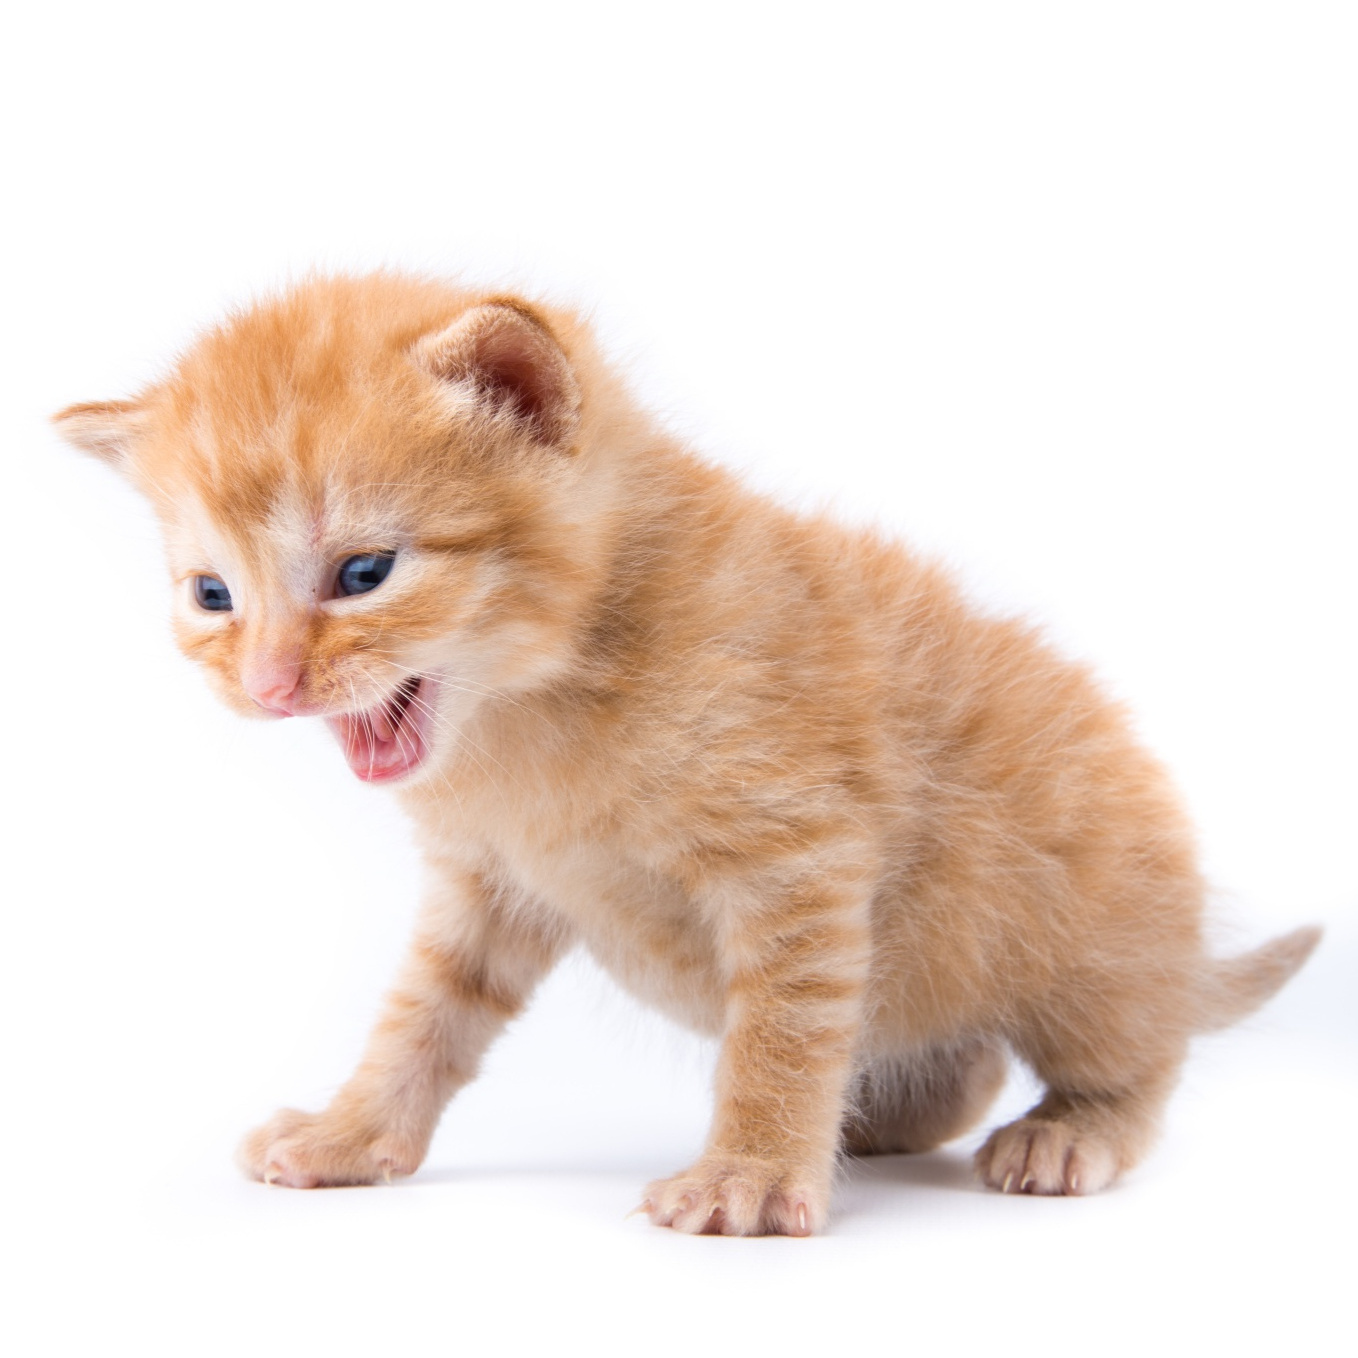
\includegraphics[width=\textwidth]{img/cat.jpg}
          \caption{Cat}\label{fig:cat}
        \end{subfigure}
        \begin{subfigure}[b]{4cm}
        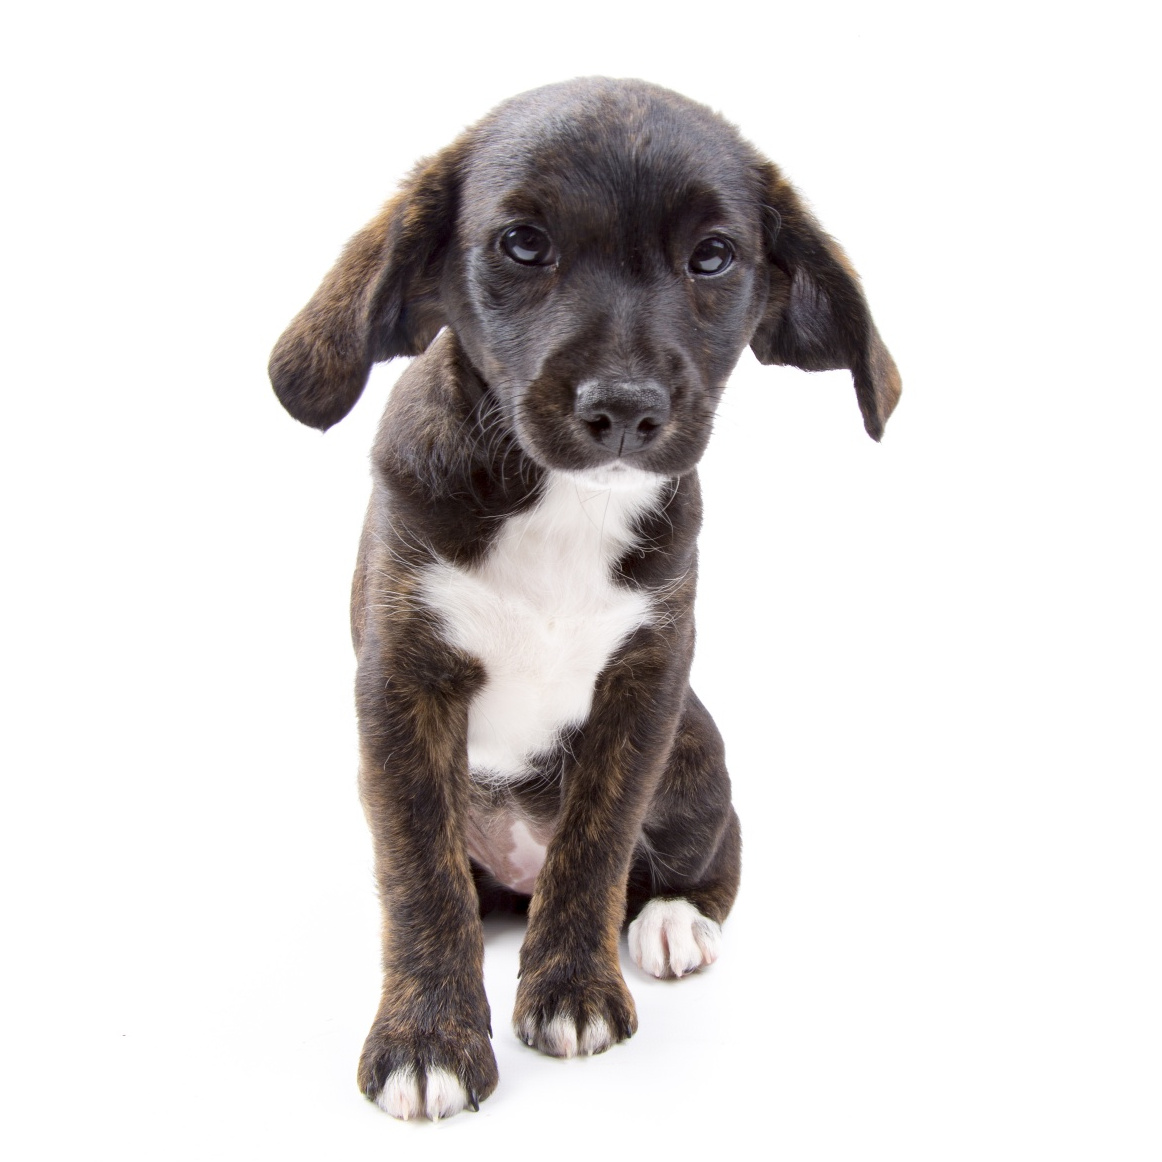
\includegraphics[width=\textwidth]{img/dog.jpg}
          \caption{Dog}\label{fig:dog}
        \end{subfigure}
        \caption{Cat and dog.}\label{fig:cat-and-dog}
      \end{figure}

    \subsection{Tables}

      Note \Cref{tab:example}.

      \begin{table}[th]
        \centering
        \begin{tabularx}{\columnwidth}{XXX}
        \toprule
        Col 1 & Col 2 & Col 3 \\
        \midrule
        Foo & Bar & Cat \\
        Short & Also short & A text that does not fit into one line and needs to be wrapped. \\
        \bottomrule
        \end{tabularx}
        \caption[Short description of a table.]{Long and very very detailed description of the table that is shown above. Yes, the description is pretty long.}\label{tab:example}
      \end{table}

    \subsection{Definitions, theorems and proofs}

      \begin{definition}[Image]
        An \( n \)-dimensional image \( f \) with \( c \) channels is a function which maps from a domain \(\Omega \subset \R^n \) to a tuple of intensity value: \( f : \Omega \to \R^c \).
      \end{definition}

      \begin{theorem}[Foo]
        All foos are bars.
      \end{theorem}
      \begin{proof}
        To prove it by contradiction try and assume that the statement is false,
        proceed from there and at some point you will arrive to a contradiction.
      \end{proof}

      \begin{lemma}[Bar]
        Most bars are also foos.
      \end{lemma}
      \begin{proof}
        Trivial.
      \end{proof}

    \subsection{Subsections and paragraphs}

      \subsubsection{This is a subsubsection}

        \paragraph{This is a paragraph} foo bar

    \subsection{Descriptions}
      \begin{description}
        \item[Optical Microscopes]
          For optical microscopy, the microscope observes the interaction between light and the matter of the sample.
        \item[Electron Microscopes]
          To take higher resolution images than possible with light an electron beam (shorter wavelength than light) is used in electron microscopy.
        \item[Scanning Probe Microscopes]
          A physical probe that scans the surface of the sample enables atomic-level resolution for scanning probe microscopy.
      \end{description}


  \section{A long text}

    \lipsum[3-56]
